\documentclass[a4paper]{article}

\usepackage{inputenc}
\usepackage[british,UKenglish]{babel}
\usepackage{amsmath}
%\usepackage{titlesec}
\usepackage{color}
\usepackage{graphicx}
\usepackage{fancyref}
\usepackage{hyperref}
\usepackage{float}
\usepackage{scrextend}
\usepackage{setspace}
\usepackage{xargs}
\usepackage{multicol}
\usepackage{nameref}

\usepackage{sectsty}
\usepackage{multicol}
\usepackage{multirow}
\usepackage[procnames]{listings}
\usepackage{appendix}

\newcommand\tab[1][1cm]{\hspace*{#1}}
\hypersetup{colorlinks=true, linkcolor=black}
\interfootnotelinepenalty=10000

\newcommand{\cleancode}[1]{\begin{addmargin}[3em]{3em}\texttt{\textcolor{cleanOrange}{#1}}\end{addmargin}}
\newcommand{\cleanstyle}[1]{\text{\textcolor{cleanOrange}{\texttt{#1}}}}


\usepackage[colorinlistoftodos,prependcaption,textsize=footnotesize]{todonotes}
\newcommandx{\commred}[2][1=]{\textcolor{Red}
{\todo[linecolor=red,backgroundcolor=red!25,bordercolor=red,#1]{#2}}}
\newcommandx{\commblue}[2][1=]{\textcolor{Blue}
{\todo[linecolor=blue,backgroundcolor=blue!25,bordercolor=blue,#1]{#2}}}
\newcommandx{\commgreen}[2][1=]{\textcolor{OliveGreen}{\todo[linecolor=OliveGreen,backgroundcolor=OliveGreen!25,bordercolor=OliveGreen,#1]{#2}}}
\newcommandx{\commpurp}[2][1=]{\textcolor{Plum}{\todo[linecolor=Plum,backgroundcolor=Plum!25,bordercolor=Plum,#1]{#2}}}

\def\code#1{{\tt #1}}

\def\note#1{\noindent{\bf [Note: #1]}}

\makeatletter
%% The "\@seccntformat" command is an auxiliary command
%% (see pp. 26f. of 'The LaTeX Companion,' 2nd. ed.)
\def\@seccntformat#1{\@ifundefined{#1@cntformat}%
   {\csname the#1\endcsname\quad}  % default
   {\csname #1@cntformat\endcsname}% enable individual control
}
\let\oldappendix\appendix %% save current definition of \appendix
\renewcommand\appendix{%
    \oldappendix
    \newcommand{\section@cntformat}{\appendixname~\thesection\quad}
}
\makeatother


% "define" Scala
\usepackage[T1]{fontenc}  
\usepackage[scaled=0.82]{beramono}  
\usepackage{microtype} 

\sbox0{\small\ttfamily A}
\edef\mybasewidth{\the\wd0 }

\lstdefinelanguage{scala}{
  morekeywords={abstract,case,catch,class,def,%
    do,else,extends,false,final,finally,%
    for,if,implicit,import,match,mixin,%
    new,null,object,override,package,%
    private,protected,requires,return,sealed,%
    super,this,throw,trait,true,try,%
    type,val,var,while,with,yield},
  sensitive=true,
  morecomment=[l]{//},
  morecomment=[n]{/*}{*/},
  morestring=[b]",
  morestring=[b]',
  morestring=[b]"""
}

\usepackage{color}
\definecolor{dkgreen}{rgb}{0,0.6,0}
\definecolor{gray}{rgb}{0.5,0.5,0.5}
\definecolor{mauve}{rgb}{0.58,0,0.82}

% Default settings for code listings
\lstset{frame=tb,
  language=scala,
  aboveskip=3mm,
  belowskip=3mm,
  showstringspaces=false,
  columns=fixed, % basewidth=\mybasewidth,
  basicstyle={\small\ttfamily},
  numbers=none,
  numberstyle=\footnotesize\color{gray},
  % identifierstyle=\color{red},
  keywordstyle=\color{blue},
  commentstyle=\color{dkgreen},
  stringstyle=\color{mauve},
  frame=single,
  breaklines=true,
  breakatwhitespace=true,
  procnamekeys={def, val, var, class, trait, object, extends},
  procnamestyle=\ttfamily\color{red},
  tabsize=2
}

\lstnewenvironment{scala}[1][]
{\lstset{language=scala,#1}}
{}
\lstnewenvironment{cpp}[1][]
{\lstset{language=C++,#1}}
{}
\lstnewenvironment{bash}[1][]
{\lstset{language=bash,#1}}
{}
\lstnewenvironment{verilog}[1][]
{\lstset{language=verilog,#1}}
{}



\graphicspath{{images/}}
\usepackage[UTF8,fontset=fandol]{ctex}
\usepackage{graphicx}
\usepackage{color,framed}
\usepackage{listings}
\usepackage{caption}
\usepackage{amssymb}
\usepackage{enumerate}
\usepackage{xcolor}
\usepackage{bm}
\usepackage{lastpage}
\usepackage{fancyhdr}
\usepackage{tabularx}
\usepackage{geometry}
\usepackage{float}
\usepackage{booktabs}
\usepackage{tikz}
\usetikzlibrary{positioning,arrows.meta,fit,backgrounds}

% 代码仅使用 listings，不需要 shell-escape 或外部高亮程序。
\lstset{
  language={},breaklines=true,basicstyle=\small\ttfamily,
  keywordstyle=\color{blue!70}\bfseries,
  commentstyle=\color{gray},stringstyle=\ttfamily,
  extendedchars=false,linewidth=\textwidth,numbers=left,
  numberstyle=\tiny\color{blue!50},frame=single,
  showstringspaces=false,columns=fullflexible
}

%-------------------------页面边距--------------
\geometry{a4paper,left=2.3cm,right=2.3cm,top=2.7cm,bottom=2.7cm}
%-------------------------页眉页脚--------------
\pagestyle{fancy}
\lhead{\kaishu\small PaperMaze}
\rhead{\kaishu\small 企业级AI软件设计与开发 · 开发设计文档}
\lfoot{}
\cfoot{\thepage}
\rfoot{}
\renewcommand{\headrulewidth}{0.1pt}
\renewcommand{\footrulewidth}{0pt}
\newcommand{\HRule}{\rule{\linewidth}{0.5mm}}
\newcommand{\HRulegrossa}{\rule{\linewidth}{1.2mm}}
\setlength{\textfloatsep}{10mm}
\setlength{\headheight}{15pt}

\begin{document}
\renewcommand{\contentsname}{目录}
\renewcommand{\appendixname}{附录}
\renewcommand{\appendixpagename}{附录}
\renewcommand{\refname}{参考文献}
\renewcommand{\figurename}{图}
\renewcommand{\tablename}{表}
\renewcommand{\today}{\number\year 年 \number\month 月 \number\day 日}

%-------------------------封面----------------
\begin{titlepage}
    \begin{center}
    
\includegraphics[width=0.8\textwidth]{NKU.png}\\[1cm]
    \vspace{20mm}
    \textbf{\huge\kaishu{软件学院}}\\[0.5cm]
    \textbf{\huge\kaishu{企业级 AI 软件设计与开发}}\\[0.5cm]
    \textbf{\Large\kaishu{综合实践 · 开发设计文档}}\\[1.3cm]
    \textbf{\Huge\kaishu{PaperMaze 纸境寻路}}\\[0.5cm]
    {\Large\kaishu{选题18：迷宫生成与寻路可视化}}\par
    \vspace{\fill}
    \centering
    {\LARGE\kaishu{学号：2311500}}\\[0.5cm]
    {\LARGE\kaishu{姓名：李锦程}}\\[0.5cm]
    \vfill
    {\Large \today}
    \end{center}
\end{titlepage}

\renewcommand{\thefigure}{\thesection.\arabic{figure}}
\counterwithin{figure}{section}
\cfoot{\thepage\ of \pageref{LastPage}}
\clearpage
\tableofcontents
\newpage

\section{项目概述与目标}

\subsection{课程背景与项目定位}
PaperMaze 纸境寻路对应“企业级 AI 软件设计与开发”综合实践的选题18：迷宫生成与寻路可视化。系统在浏览器中生成迷宫，支持手动探索、编辑墙体与起终点，并通过广度优先搜索（BFS）与 A* 观察搜索过程、最短路径与运行指标，最终将运行结果连同完整地图快照保存在本地。

本项目面向单机单用户的课堂演示环境，前端采用 Vue 3、TypeScript 与 SVG 构建交互界面，后端采用 Python FastAPI 提供接口，底层由 SQLite 保存数据。此处“企业级”仅为课程名称，不表明该课程原型已具备多用户、分布式部署或生产运维能力。运行时 AI 解读属于可选辅助功能，未配置 API 密钥时，系统仍可独立完成迷宫生成、探索、寻路求解及数据存盘与恢复。

\subsection{开发目标与主流程}
系统重点打通“生成或编辑迷宫—手动探索或运行算法—观察对比结果—本地保存—刷新后完整恢复”的端到端闭环。围绕该主流程，主要设计目标如下：
\begin{enumerate}
  \item 使生成逻辑、移动规则与搜索过程透明可查，避免仅展示预设动画。
  \item 在同一张地图上对齐 BFS 与 A*，以真实运行数据对比路径长度、遍历节点数及算法耗时。
  \item 保存完整地图快照，使手动编辑后的地图和结果能够跨页面刷新恢复。
  \item 提供明确的无解反馈、输入校验、保存失败重试及 AI 降级机制，保障核心流程稳定。
  \item 在课程规模内保持模块职责清楚，便于现场说明代码、算法与验证依据。
\end{enumerate}

\subsection{文档依据与范围}
本文以 \path{SOURCE_design.md} 为主要依据，并与 \path{ARCHITECTURE.md}、\path{AI_USAGE.md}、\path{ACCEPTANCE_CHECKLIST.md}、\path{README.md} 及 \path{TESTING.md} 进行交叉比对。文中所列测试数据、运行截图与历史验收结论均直接引用上述材料，不代表编写本文档时重新执行了全量测试。针对 \path{README.md} 中出现的“数据结构课程综合实践”表述，本文统一采用当前提交所要求的课程名称；具体功能范围仍严格以随附工程材料为准。

\clearpage
\subsection{成品界面概览}
\begin{figure}[H]
  \centering
  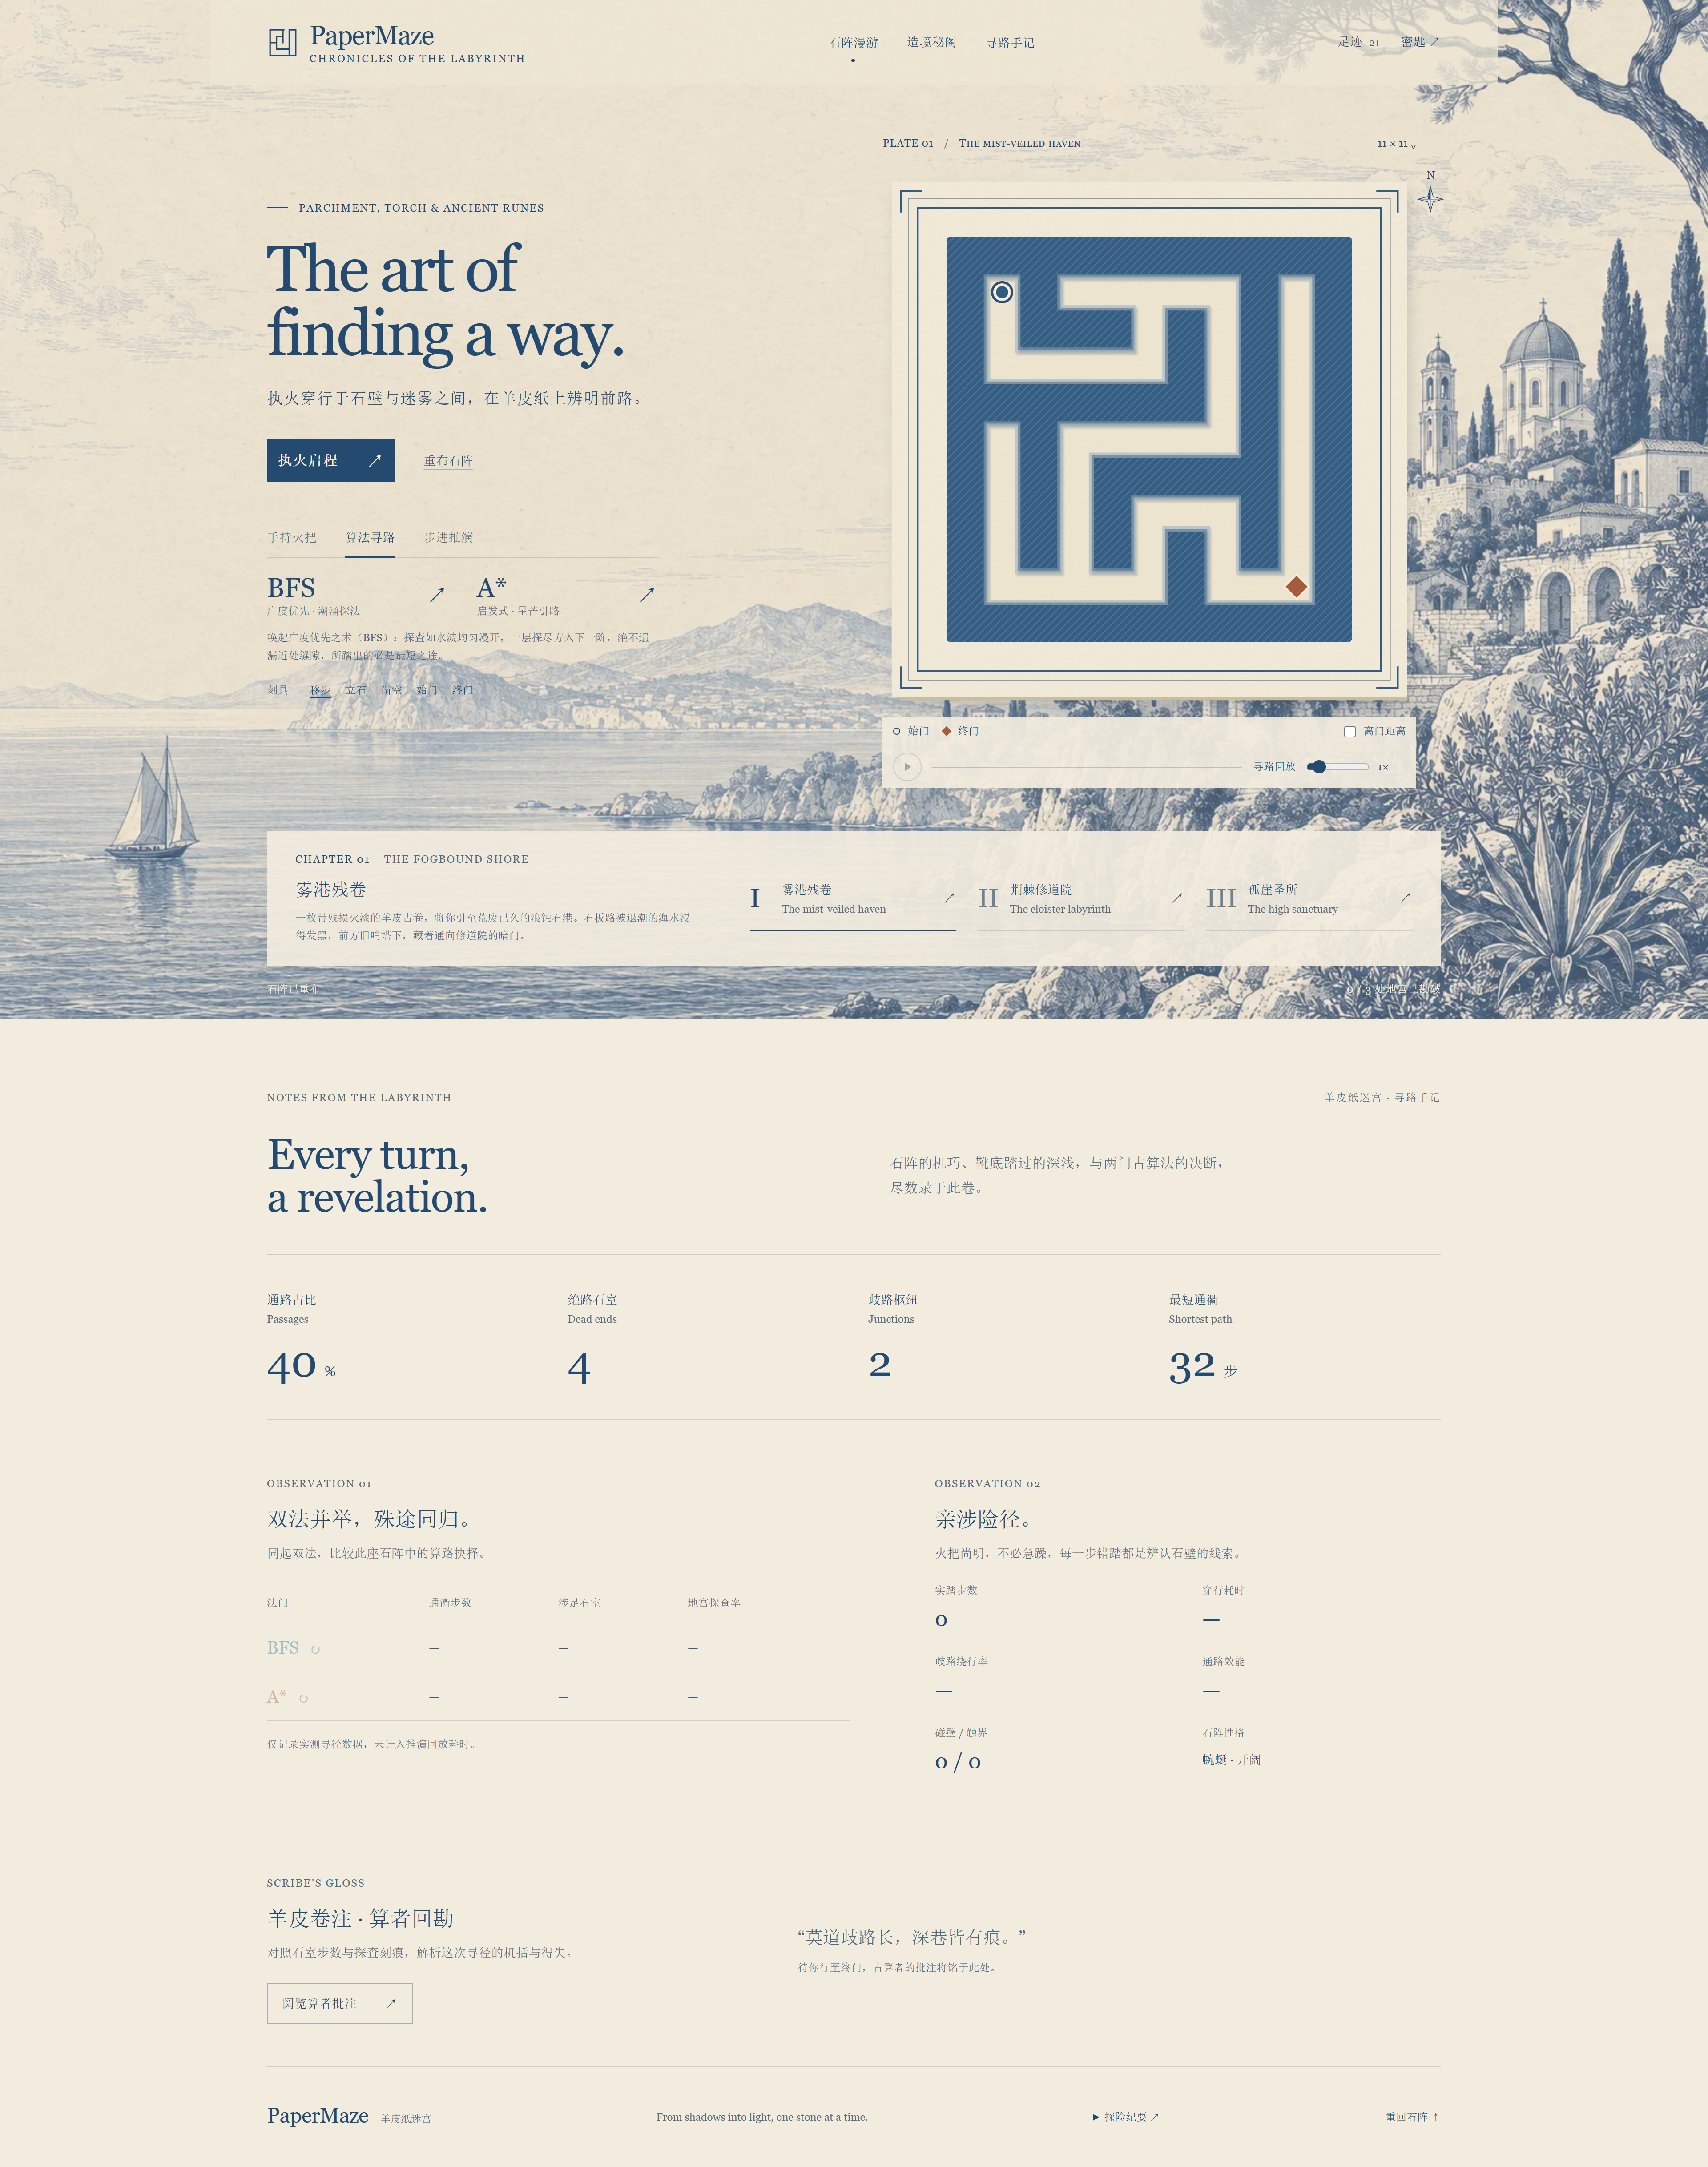
\includegraphics[width=\textwidth,height=0.78\textheight,keepaspectratio]{00-整体页面.png}
  \caption{PaperMaze 完整主页面（11×11，种子123）}
  \label{fig:workbench}
\end{figure}
图\ref{fig:workbench} 为本次在运行应用中实拍的完整页面：上部为故事场景、探索方式与 SVG 迷宫，下部为寻路手记、结构指标和解读入口。截图采用 1920×1080 视口、2 倍设备像素比，并包含视口以下内容。
\clearpage

\section{需求分析}

\subsection{基础需求与扩展需求}
选题要求系统具备随机生成与重置迷宫、指定起点和终点、响应键盘与按钮控制移动、实时判定碰撞与边界、运行寻路算法并高亮路径、统计路径长度、节点访问数和耗时，以及妥善处理无解情况的能力。课程统一规范还要求服务稳定启动、核心业务逻辑真实生效、数据持久化闭环完整，并具备基本的异常防御能力。

\begin{table}[htbp]
\centering
\caption{功能需求及对应设计}
\small
\begin{tabularx}{\textwidth}{p{2.2cm}X}
\toprule
功能 & 实现范围 \\
\midrule
迷宫生成 & 支持 11、21、31、41、51 五档方形网格；支持种子确定性复现；可视化演示 DFS、随机 Prim 与 Kruskal 生成过程。\\
手动探索 & 支持方向键、WASD 与屏幕软键盘；校验合法移动，记录碰撞次数并在抵达终点时结算成绩。\\
地图编辑 & 支持自定义切换起点、终点、墙体与通道；锁定保护外围边界，校验起终点合法性。\\
算法寻路 & 支持 BFS 与 A*；支持同图对比；采集搜索轨迹、最短路径、访问节点数与纯计算耗时。\\
可视化与教学 & 支持动画暂停、重播与倍速调节；支持事件级单步推演与回退；提供拓扑指标与终点距离热力图。\\
历史记录 & 支持记录保存、列表展示、模式筛选、状态恢复与记录删除；完整保存编辑后的地图矩阵。\\
AI 解读 & 后端按需请求 DeepSeek 接口；未配置密钥或网络异常时自动降级为本地规则分析。\\
\bottomrule
\end{tabularx}
\end{table}

\subsection{使用场景与约束}
用户可使用固定种子生成初始迷宫并手动试走，随后运行算法将个人行进路线与最短路径进行比对；亦可在线编辑迷宫，观察新增障碍、封闭环路或断开通路对算法决策的影响。教学模式旨在逐步拆解待选队列更迭、父节点指针回溯以及 A* 代价函数计算细节；生成器工作台则用于动态观察迷宫开凿过程。

界面采用纸艺剪影风格的 SVG 图形与三幕式场景构建交互，场景过渡对应 DFS、Prim 和 Kruskal 三种生成机制，场景叙事要素不参与实际算法计算。通关章节标记存储于浏览器本地 localStorage，完整运行记录与地图快照则写入 SQLite，二者分工明确。

非功能性约束包括：寻路计算不得变更输入地图数据；算法运行耗时不计入界面渲染与网络传输延迟；若后端服务离线，前端已加载页面中的迷宫生成、移动及搜索运算仍应正常执行；系统支持的最大尺寸标定为 51×51，以目标浏览器的实测渲染表现为准。

\section{设计理念}

\subsection{以三幕故事引导算法学习}
PaperMaze 将算法实验组织为欧洲奇幻背景下的“三幕纸上旅程”，而不是将故事当作独立于操作的装饰。\path{frontend/src/scenes.ts} 定义了“雾港残卷”“荆棘修道院”“孤崖圣所”三幕，分别绑定 DFS 回溯、随机 Prim、Kruskal 并查集生成方式。用户从海港的残卷出发，经修道院走向峭壁上的圣所；\path{App.vue} 展示各幕叙事、发现提示与通关结语，手动抵达终点后可继续下一章，也可通过场景导航切换。故事解释探索情境，地图与路径仍由真实算法计算，不由剧情预设。

学习路线由浅入深：先切换“手持火把”，用方向键或 WASD 亲自试走，感受岔路、碰壁与绕行；再切换“算法寻路”，在同一地图上观察 BFS 的逐层扩展与 A* 的启发式选择，并在“寻路手记”比较实际指标；最后进入“步进推演”，用前进、回退观察候探队列、父指针和 A* 的 $g/h/f$。这种组织方式把探索中产生的疑问带入算法对比，再落到可检查的单步状态，而不宣称已验证学习效果。

\subsection{旧纸与钴蓝蚀刻的统一界面}
\path{README.md} 与 \path{frontend/src/style.css} 中的旧纸底色、蓝色字线和欧式版画场景，构成地图册式的视觉语言。场景插画由 \path{scenes.ts} 引用独立 WebP 资源；\path{PaperLayers.vue} 用 SVG 纸层切口、两层阴影、斜线蚀刻和纸纹呈现墙体，\path{MazeBoard.vue} 叠加路线、访问点与终门标记。故事里的“火把”“刻具”“足迹”对应手动移动、地图编辑和历史恢复等真实操作。风格负责保持旅程的连贯性，计算、指标与持久化边界则保持清楚，不把场景动效当作算法运行。

\section{总体架构}

\subsection{分层与数据流}
系统由前端单页应用、后端 HTTP 接口与本地轻量数据库构成。交互层调用 TypeScript 纯函数获取计算结果，交由播放调度器与 SVG 渲染组件呈现；保存数据时，前端组装 JSON 运行摘要与快照，由 FastAPI 服务端校验后持久化至 SQLite。历史记录恢复时，直接通过详情接口拉取完整快照重构地图，而非仅依赖随机种子重新演算。

\begin{figure}[htbp]
\centering
\begin{tikzpicture}[
  font=\small, >=Latex,
  box/.style={draw=blue!45!black,rounded corners=2pt,fill=white,align=center,inner sep=6pt},
  flow/.style={->,thick,draw=blue!55!black},
  layer/.style={draw=blue!35!black,rounded corners=3pt,fill=blue!3,inner sep=9pt}
]
  \node[box,text width=13.4cm] (ui) {\textbf{前端表现层 · Vue 3}\\
    \texttt{App.vue}：操作、场景与历史编排；\texttt{scenes.ts}：三幕叙事\\
    \texttt{usePlayback.ts}：结果回放；\texttt{useTeachingPlayback.ts}：事件游标\\
    \texttt{MazeBoard.vue}、\texttt{PaperLayers.vue}：SVG 地图与纸层渲染};

  \node[box,text width=2.8cm,minimum height=1.45cm,below=1.2cm of ui,xshift=-5.1cm] (gen)
    {迷宫生成\\{\scriptsize\texttt{core/generator.ts}}\\DFS / Prim / Kruskal};
  \node[box,text width=2.8cm,minimum height=1.45cm,right=0.17cm of gen] (move)
    {移动与编辑\\{\scriptsize\texttt{core/maze.ts}}\\坐标规则、挑战码};
  \node[box,text width=2.8cm,minimum height=1.45cm,right=0.17cm of move] (search)
    {BFS 与 A* 寻路\\{\scriptsize\texttt{core/search.ts}}\\结果、教学事件};
  \node[box,text width=2.8cm,minimum height=1.45cm,right=0.17cm of search] (analysis)
    {结构分析\\{\scriptsize\texttt{core/analysis.ts}}\\指标、终点距离场};
  \begin{scope}[on background layer]
    \node[layer,fit=(gen)(analysis),label={[anchor=south west,font=\small\bfseries]north west:前端领域层 · 纯 TypeScript}] (domain) {};
  \end{scope}
  \draw[flow,<->] (ui.south) -- node[right,font=\scriptsize,fill=white] {函数调用 / 真实结果与事件} (domain.north);

  \node[box,text width=6cm,minimum height=1.6cm,below=1.1cm of gen.south west,anchor=north west] (api)
    {\textbf{FastAPI · \texttt{backend/main.py}}\\
     \texttt{/api/runs}：Pydantic 校验、历史接口\\
     \texttt{/api/ai/explain}：校验解读指标};
  \node[box,text width=6cm,minimum height=1.6cm,right=0.35cm of api] (ai)
    {\textbf{AI 解读 · \texttt{backend/main.py}}\\
     DeepSeek（仅后端读取密钥）\\
     无密钥或上游异常：本地规则兜底};
  \draw[flow,<->] (api) -- (ai);
  \draw[flow,<->] (ui.west) -- ++(-0.55,0) |- (api.west);
  \node[font=\scriptsize,rotate=90,fill=white] at ([xshift=-0.55cm,yshift=-2.7cm]ui.west) {\texttt{api.ts}: JSON / HTTP};
  \node[box,text width=12.8cm,below=0.65cm of api.south west,anchor=north west] (db)
    {\textbf{SQLite · \texttt{backend/storage.py}}\\
     \texttt{runs} 表：索引字段 + 完整 JSON 运行快照（含编辑后地图、起终点与结果）};
  \draw[flow,<->] (api.south) -- (api.south |- db.north);
\end{tikzpicture}
\caption{依据实际源文件绘制的分层架构与数据流}
\label{fig:architecture}
\end{figure}
图\ref{fig:architecture} 中，领域函数在浏览器内执行；HTTP 箭头连接界面编排与后端，不表示将寻路计算交给服务器。AI 解读返回文本，SQLite 保存运行快照，二者不共用持久化流程。

\subsection{模块职责}
\begin{table}[htbp]
\centering
\caption{主要模块与职责边界}
\small
\begin{tabularx}{\textwidth}{p{5.1cm}X}
\toprule
模块（前端路径相对 \texttt{frontend/src/}） & 职责 \\
\midrule
\texttt{core/maze.ts} & 地图表示、确定性生成入口、移动与编辑规则、挑战码。\\
\texttt{core/generator.ts} & 三类迷宫生成算法、不可变快照、结构指标与生成事件。\\
\texttt{core/search.ts} & BFS、A*、路径校验、教学事件与状态重放。\\
\texttt{core/analysis.ts} & 迷宫结构指标与终点距离场计算。\\
\texttt{usePlayback.ts} & 搜索结果的访问阶段与路径阶段回放。\\
\texttt{useTeachingPlayback.ts} & 过程事件游标、单步、回退、自动播放与重置。\\
\texttt{MazeBoard.vue}、\texttt{PaperLayers.vue} & 地图、搜索层、热力图及纸层 SVG 渲染。\\
\texttt{App.vue}、\texttt{scenes.ts} & 组织交互与场景切换，清理跨地图旧状态。\\
\texttt{backend/main.py} & HTTP 接口、输入校验与静态页面服务。\\
\texttt{backend/storage.py} & 负责 SQLite 运行记录的保存、查询与删除。\\
\bottomrule
\end{tabularx}
\end{table}

\subsection{核心设计取舍}
\begin{itemize}
  \item \textbf{求解与播放分离：}算法运算与视觉回放解耦。寻路首先完成纯数据计算，再由播放器调度渲染动画；中途暂停、变速或发起存盘均不影响既定结果与算法耗时统计。
  \item \textbf{优先持久化完整快照：}种子仅能重现初始迷宫，无法反映用户后续的手工编辑；运行历史完整保存整幅二值矩阵与起终点坐标。
  \item \textbf{同图比对状态独立：}两种算法基于同一份不可变地图数据运行，各自维护私有的待选队列、访问集合、代价字典与父指针映射，杜绝搜索状态相互干扰。
  \item \textbf{轻量化技术选型：}依托前端原生能力与本地 SQLite，不针对小规模演示引入复杂的外部服务、ORM 框架或数据库迁移中间件。
  \item \textbf{AI 不阻断主流程：}密钥只由后端读取，解读失败时使用本地规则，算法指标始终来自本地计算。
\end{itemize}

\section{核心模块设计}

\subsection{迷宫表示与生成}
迷宫以二维矩阵建模，数值 0 代表通路，1 代表墙体。运行时快照涵盖网格规格、随机种子、生成器类型、起终点坐标、编辑修改标记及完整二值矩阵。在生成算法、网格尺寸与随机种子一致的前提下，能够复现初始地图。

深度优先搜索（DFS）生成器从预设起点出发，随机挑选未探索的网格单元并打通阻隔墙体，遭遇死胡同则逐层回溯；随机 Prim 算法维护待处理前沿边界集合，逐步吸纳邻接单元以扩展连通图；Kruskal 算法则借助并查集管理连通分量，通过有序连通不相交集合形成迷宫。生成模块对外输出最终静态快照以及完整的生成事件流，供动效播放器消费；回退推演时仅移动游标位置，不直接修改底层核心矩阵。

挑战码用于在客户端间共享初始状态：早期格式形如 \texttt{PM1-尺寸-种子}（默认绑定 DFS），现行扩展格式为 \texttt{PM2-算法-尺寸-种子}，显式记录生成器类型。挑战码不承载后续编辑操作，包含人工编辑的地图须通过历史快照恢复。

\begin{figure}[htbp]
  \centering
  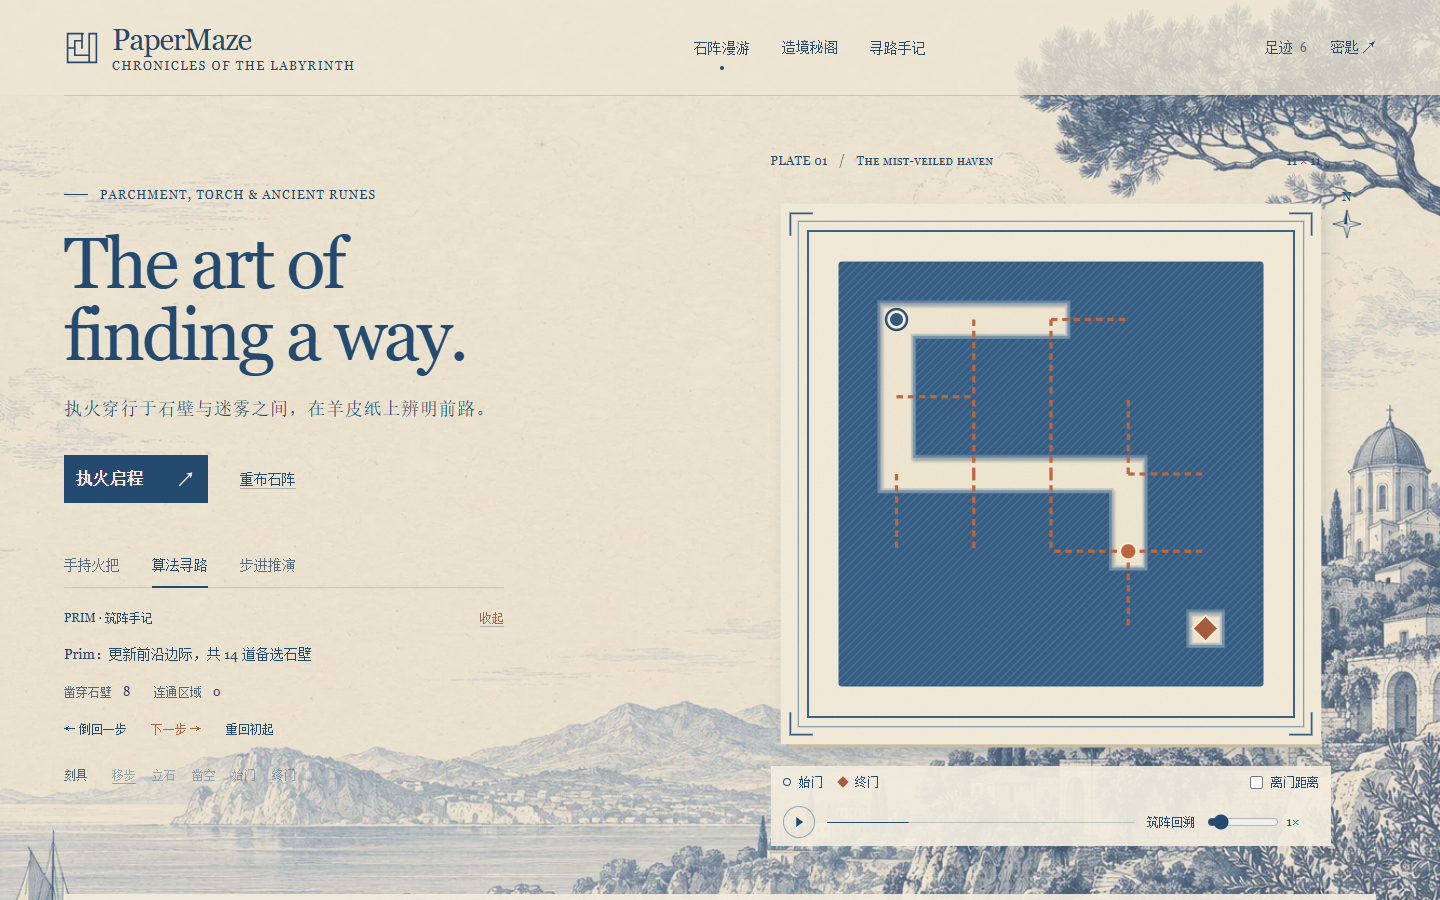
\includegraphics[width=\textwidth,height=0.46\textheight,keepaspectratio]{07-生成过程.png}
  \caption{随机 Prim 的逐步开凿过程}
  \label{fig:generation}
\end{figure}
图\ref{fig:generation} 呈现了真实生成轨迹中的游标状态：浅色单元表示已连通区域，虚线标注当前候选边，底部滑块控制演播速率。逻辑单元计数、开凿边数、连通分量状态及环路秩均实时取自底层算法数据。

\subsection{手动探索与地图编辑}
手动探索依据方向输入更新目标网格位置。若目标坐标越界或落在墙体内，系统拦截位移，保留原地坐标并增加碰撞计数；只有合法移动才会将坐标推入行进轨迹序列，碰撞行为不计入行进有效步数。操作支持物理方向键、WASD 键与屏幕虚拟按键，成功抵达终点后触发结算逻辑，保存路线轨迹、总耗时与碰撞频次。中途放弃的探索不会生成通关有效记录。

地图编辑模式支持动态修改起点、终点位置，以及在空地和墙体间切换。系统强制保护外围边界墙不可擦除，禁止起终点坐标重叠，且起终点不可落于墙体上。在生成新地图、修改地形或切换场景时，调度器自动终止当前播放进程并清理残留轨迹，防止旧地图数据污染新画布。

\begin{figure}[htbp]
  \centering
  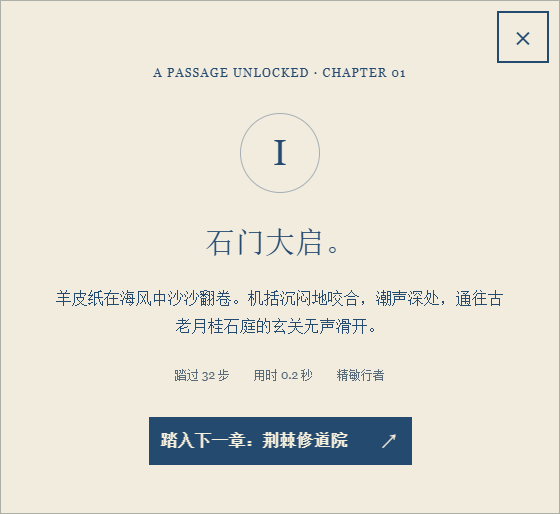
\includegraphics[width=\textwidth,height=0.46\textheight,keepaspectratio]{03-手动通关.png}
  \caption{手动到达终点后的结果窗口}
  \label{fig:manual}
\end{figure}
图\ref{fig:manual} 截取自自动化测试脚本按既定路线模拟按键后的通关弹窗，界面耗时反映测试脚本调用间隔，不代表人工实测挑战成绩。

\subsection{BFS 与 A* 寻路}
BFS 以队列按层扩展通路节点，在四方向、单位代价的网格中得到最短步数路径。A* 按估价函数选择候选节点：
\[
  f(n)=g(n)+h(n),\qquad h(n)=|x_n-x_t|+|y_n-y_t|.
\]
其中 $g(n)$ 代表从起始点到当前节点的已知最小步数，$h(n)$ 采用终点曼哈顿距离作为启发式估计。两种算法分别记录各自的父节点索引，搜索成功后沿指针反向回溯生成路径，并严格校验首尾端点、通路连通性及相邻节点间距。终点不可达时规范返回空路径，不构建虚假连接。

A* 算法支持对已发现节点的更优路径更新机制：当经由新节点发现到达已入队节点的 $g$ 值更小时，系统刷新该节点的代价与父节点指针，并重新调整其在优先队列中的排序位置。所供材料记录了一个编辑后带环地图的反例：修复前 BFS 为16步、A* 为18步；修复后均为16步。该问题说明不能将“已经发现”误当作“当前代价不再需要更新”。

常规搜索输出由最终路径、访问序列、连通标识与性能指标构成；教学推演事件流由独立管道生成与维护，二者不能混用同一动画游标。

\subsection{可视化、回放与教学}
SVG 渲染层将迷宫实体墙转化为多层纸质剪影，并依次叠加手动行进路线、双算法对比图层与距离热力渐变。纹理与阴影滤镜挂载于图层全局，点击事件通过 SVG 变换矩阵逆运算映射为精准的网格坐标。生成过程回放基于打通的边列表重构局部渲染矩阵，底层领域快照保持只读。

寻路过程遵循“先运算、后展播”的模式，播放控制器将动画拆分为节点遍历扩展阶段与最优路径描摹阶段，支持随时暂停、重放以及 0.5×--5× 范围内的倍速控制（滑块步进 0.5×）。动效播放依据时间增量平滑插值，单帧内可步进渲染多个节点；当前选中的算法展示动态扩展细节，对比算法则以静态透明层保留轮廓以供对照。

教学模式完整捕获了微观事件流，配合双向游标支持单步步进、步退、自动推演、中断与重置。面板实时呈现开放队列清单、当前聚焦节点、父子指针关系以及 A* 算法对应的 $g/h/f$ 数值。教学与生成事件流仅在活跃会话的内存中维护，持久化时不保存逐帧数据；重新加载历史时根据快照重新计算所需轨迹。

\begin{figure}[htbp]
  \centering
  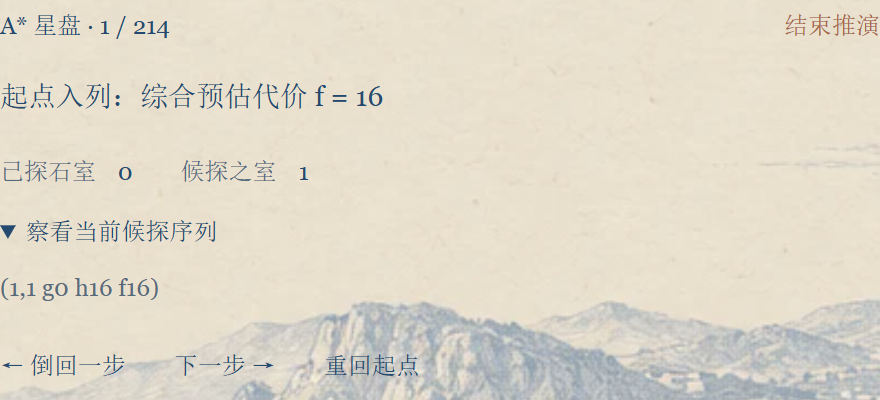
\includegraphics[width=\textwidth,height=0.46\textheight,keepaspectratio]{06-教学推演.png}
  \caption{A* 教学推演中的候选序列与代价}
  \label{fig:teaching}
\end{figure}

\subsection{持久化与历史恢复}
SQLite 数据库中的 \texttt{runs} 表用于持久化运行数据，包含记录唯一标识、运行模式、入库时间戳及全量 JSON 负载。该负载完整存储地图快照、连通状态、最终路径、节点展开序列及对应性能指标；系统默认数据库文件位于工程根目录下的 \texttt{papermaze.sqlite3}。结构中通过 \texttt{schemaVersion} 与 \texttt{generatorVersion} 字段维护版本兼容性；当解析未记录生成器类型的老版本数据时，默认按 DFS 策略兼容读取。

\begin{table}[htbp]
\centering
\caption{运行历史接口契约}
\small
\begin{tabularx}{\textwidth}{p{5.1cm}X}
\toprule
接口 & 职责与边界 \\
\midrule
\texttt{POST /api/runs} & 写入运行记录；相同 ID 且内容一致时幂等返回原数据，相同 ID 但数据冲突时返回409。\\
\texttt{GET /api/runs} & 获取历史记录摘要列表，支持按模式分类筛选。\\
\texttt{GET /api/runs/\{id\}} & 获取指定记录的全量快照与结算数据，供界面复盘与重播。\\
\texttt{DELETE /api/runs/\{id\}} & 移除指定运行记录；记录未命中时返回404。\\
\bottomrule
\end{tabularx}
\end{table}

保存操作由前端发起，后端依赖 Pydantic 校验模型对尺寸范围、矩阵规格、起终点有效性、路径连续性、访问轨迹结构以及各项统计指标进行严格验证后方可落盘。在复现历史时，系统直接读取数据库中存储的完整矩阵与起终点坐标，不依靠重新随机生成。

\begin{figure}[htbp]
  \centering
  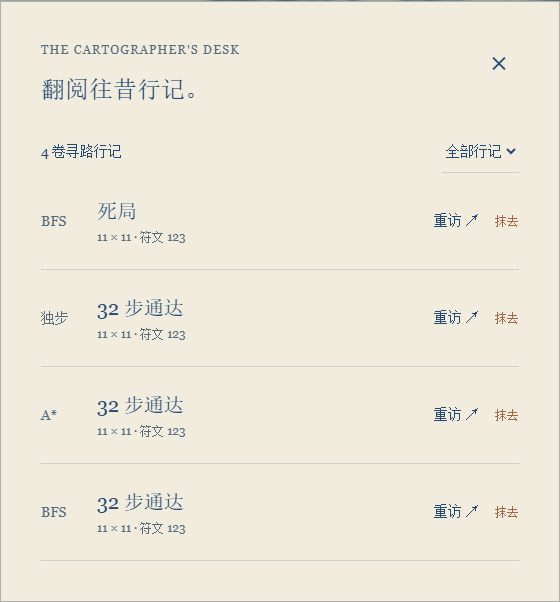
\includegraphics[width=\textwidth,height=0.46\textheight,keepaspectratio]{05-运行历史.png}
  \caption{刷新后查看运行历史并重访完整快照}
  \label{fig:history}
\end{figure}
图\ref{fig:history} 取自独立测试环境下的数据库实例，其中包含无解探索、手动挑战及多组算法对比记录。配套测试套件对恢复后的地图矩阵和起终点进行了逐格比对，验证了数据还原的准确性。

\section{关键业务规则}

\subsection{地图一致性与结果生命周期}
单次寻路或探索严格绑定不可变地图快照。BFS、A* 及手动探索统一遵循网格坐标约定；进行同图性能评测时，锁定当前地图后分别初始化独立的搜索上下文。重新生成迷宫、手动编辑网格或切换叙事场景时，系统即刻终止既有动画并注销旧有结果，防止跨地图的快照、行进轨迹与性能统计混淆。种子与挑战码仅定义初始生成状态，编辑修改后的权威数据以存储载荷中的完整二值矩阵为准。

\subsection{指标口径}
\begin{itemize}
  \item \textbf{路径长度：}成功寻得路径时定义为路径坐标节点数减一；终点不可达时规范标识为无解，禁止将空路径误计为有效长度。
  \item \textbf{访问节点数：}来自实际出队的搜索轨迹，既不是动画帧数，也不是教学事件数。
  \item \textbf{算法耗时：}在纯搜索函数内部计时，不包含播放、暂停、网络请求和数据库保存。
  \item \textbf{手动步数：}仅累加有效的位移操作步数，碰撞行为独立记录；只有成功抵达终点方可结算为通关记录。
\end{itemize}
在存在可用最优解且用户成功通关的前提下，设用户手动步数为 $L_m$，算法最短步数为 $L_s$，定义：
\[
  \text{绕路率}=\frac{L_m-L_s}{L_s},\qquad
  \text{路线效率}=\frac{L_s}{L_m}.
\]
若算法判定迷宫无解或用户未能通关，不计算上述效率指标。

\begin{figure}[htbp]
  \centering
  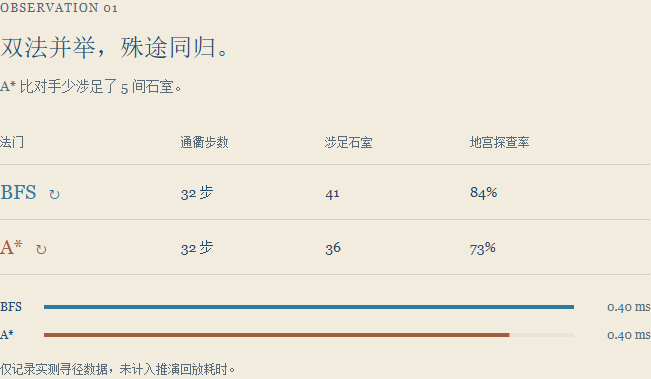
\includegraphics[width=\textwidth,height=0.46\textheight,keepaspectratio]{02-指标比较.png}
  \caption{固定示例的 BFS 与 A* 实际指标比较}
  \label{fig:metrics}
\end{figure}
图\ref{fig:metrics} 记录了一次典型运行实例：两种算法均得到32步路径，BFS 访问41个节点，A* 访问36个节点。该结果只适用于本次地图及运行，不能据此断言 A* 在所有地图都更快；单次耗时还受设备和浏览器状态影响。

\section{异常处理}

\begin{table}[htbp]
\centering
\caption{主要异常及处理方式}
\small
\begin{tabularx}{\textwidth}{p{3.1cm}X}
\toprule
异常 & 处理方式 \\
\midrule
非法尺寸或种子 & 限制输入范围；后端拒绝不符合尺寸和矩阵约束的载荷。\\
撞墙或出界 & 拦截玩家坐标位移，递增碰撞计数器，不计入有效行进位移。\\
非法地图编辑 & 拦截对外围边界墙的修改，禁止重叠或将起终点置于墙体；变更后废除旧解。\\
终点不可达 & 明确标识无解状态，输出空路径结构，系统支持如实持久化无解搜索记录。\\
非法历史载荷 & 路径不连通或地图校验未通过时返回422状态码，拒绝脏数据写入底层数据库。\\
数据冲突或缺失 & 相同 ID 数据冲突时返回409状态码；请求不存在的记录 ID 时返回404状态码。\\
后端服务离线 & 前端暂存待提交数据并提示重试；纯前端的迷宫生成、编辑与求解正常可用。\\
AI 服务异常 & 密钥缺失、网络超时、上游接口报错或响应格式异常时，自动平滑降级至本地规则。\\
\bottomrule
\end{tabularx}
\end{table}

\begin{figure}[htbp]
  \centering
  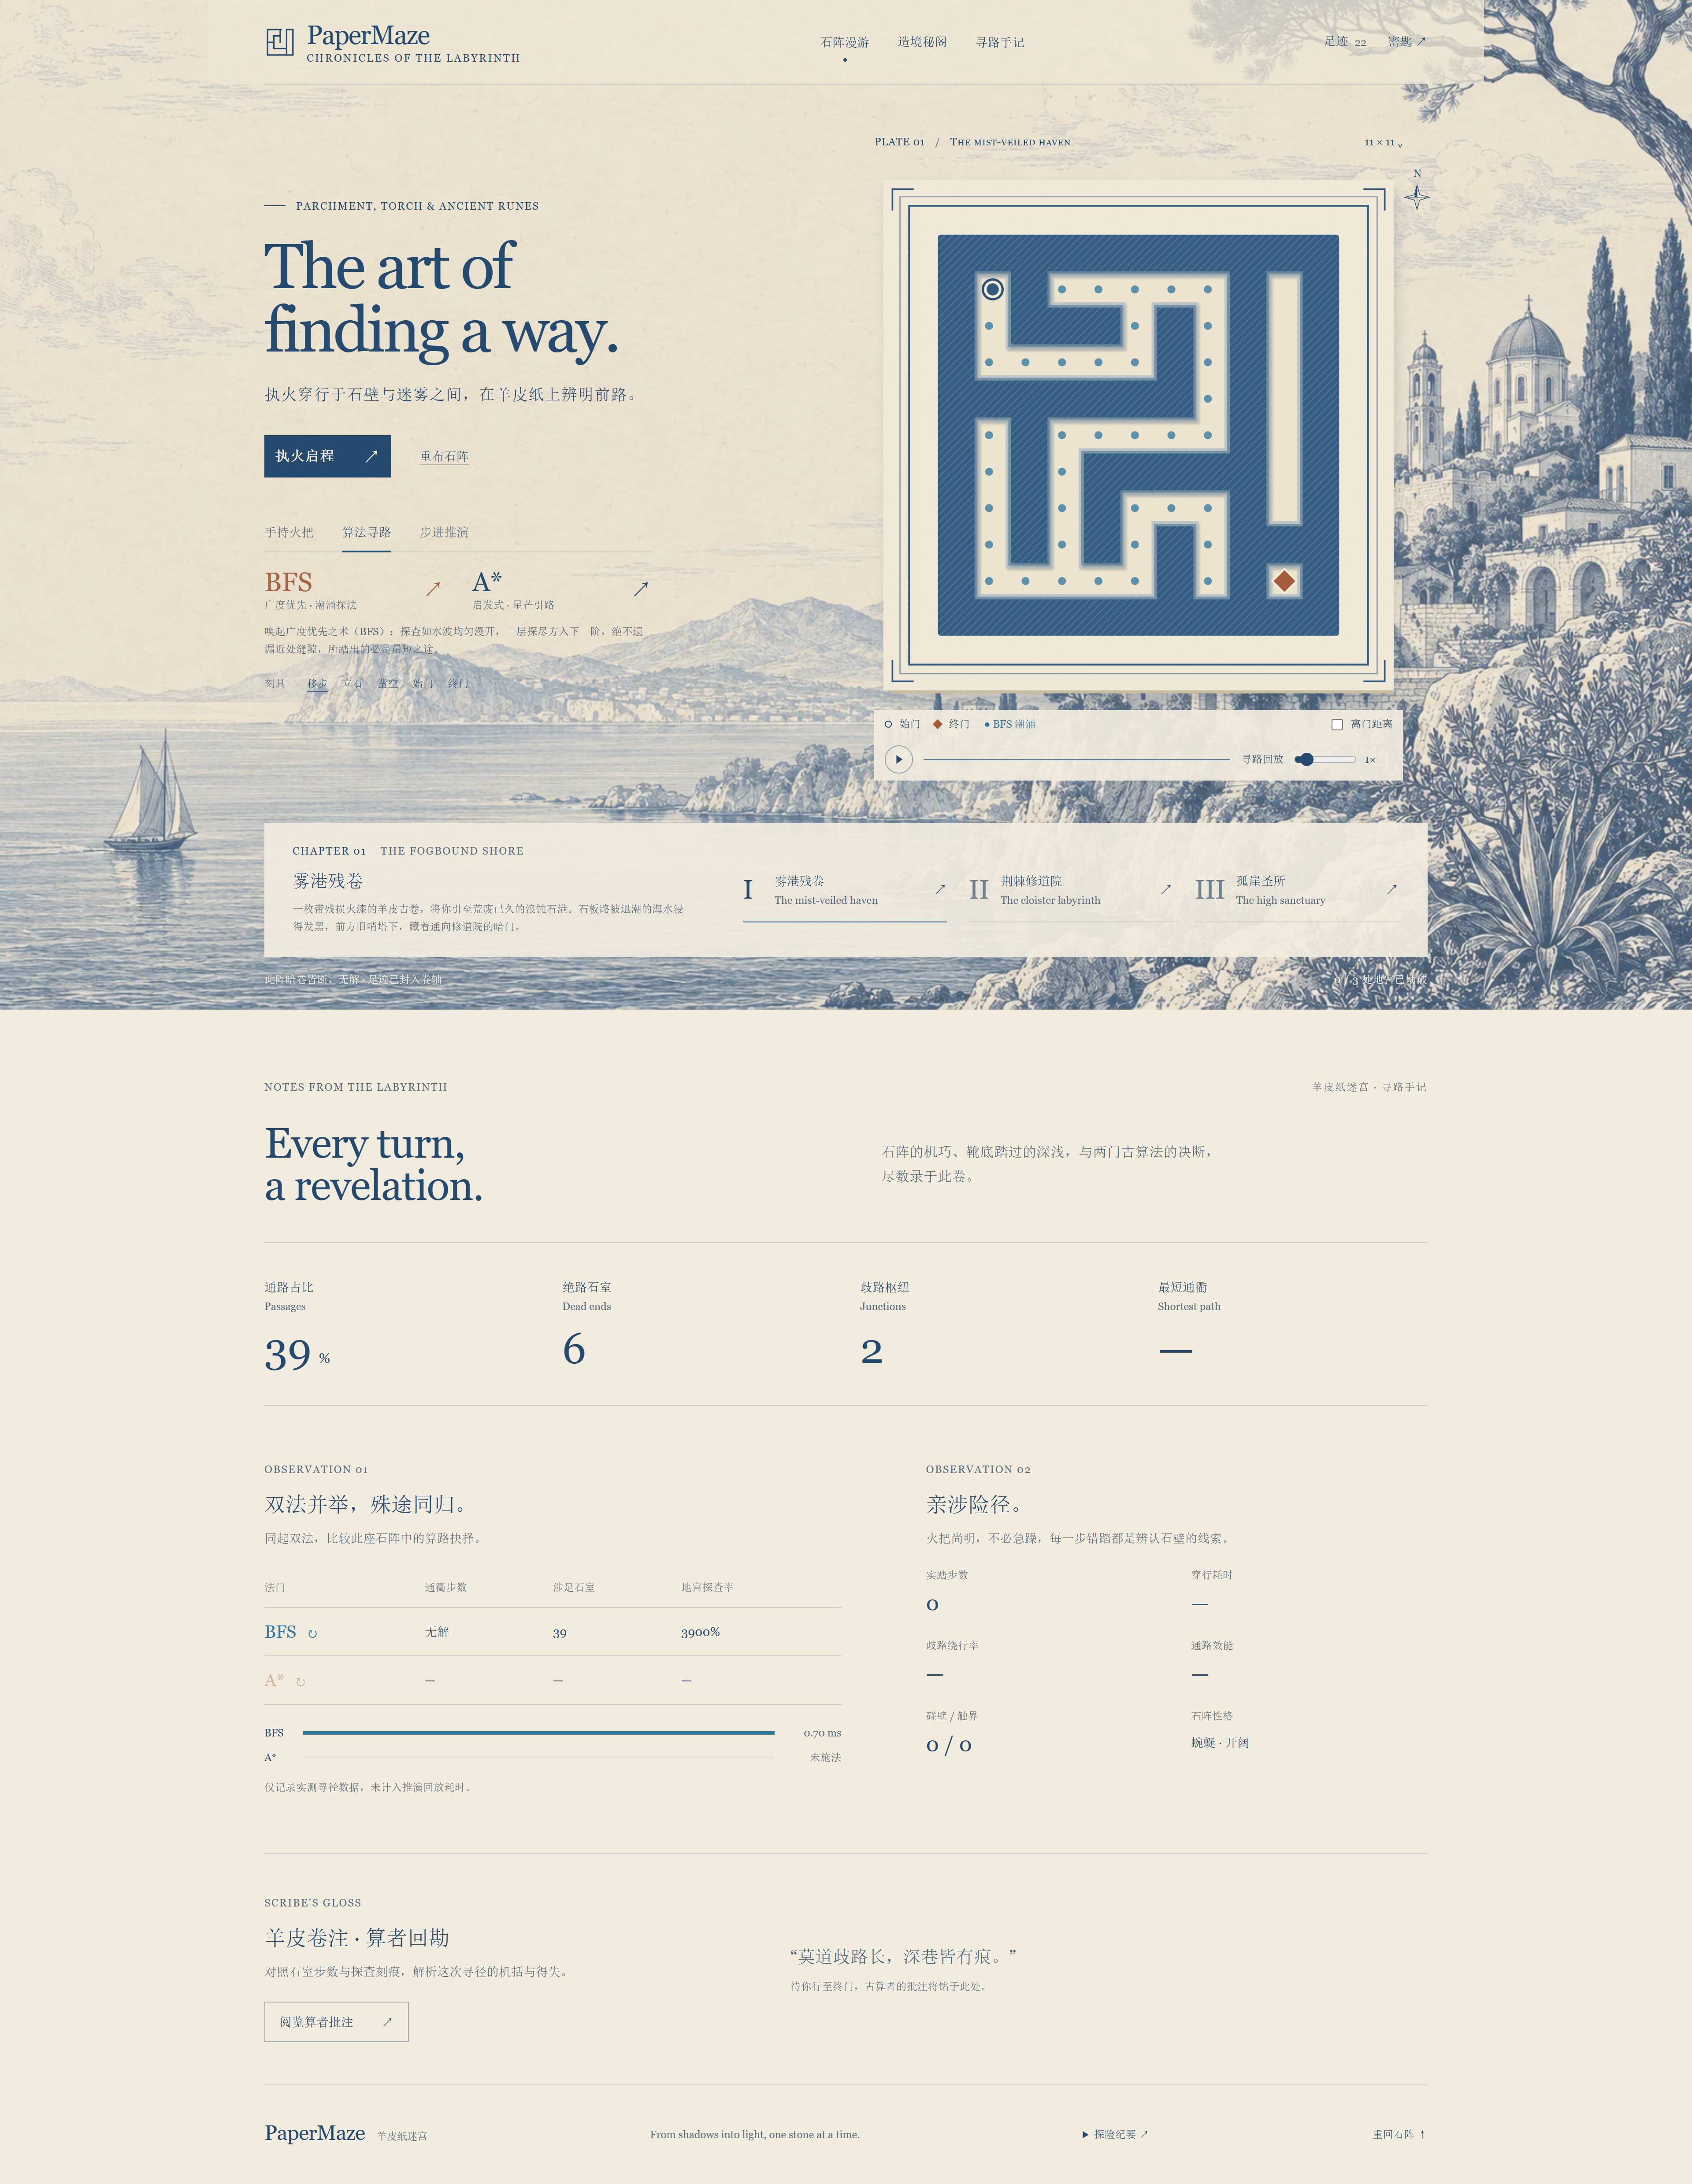
\includegraphics[width=\textwidth,height=0.76\textheight,keepaspectratio]{04-无解提示.png}
  \caption{编辑地图后的无解提示}
  \label{fig:unreachable}
\end{figure}
在迷宫寻路场景中，终点不可达属于正常的边界计算输出，不应视作系统故障。图\ref{fig:unreachable} 为本次真实操作截图：在 11×11、种子123的地图中用“立石”封闭终门的两个内部相邻格，另两侧为外围墙，再运行 BFS。终门仍为通路格，但四邻均为墙；页面显示“此阵暗巷皆断，无解”，BFS 返回空路径并访问39个节点。截图脚本及接口核验摘要保留在 \path{scripts/capture_pages.py} 与 \path{scripts/capture_evidence.json}。截图中的探查率显示异常属于现有界面问题，不作为正确指标引用，本次未修改应用源码。

\section{测试与验收}

\subsection{测试层次与验证重点}
自动化测试主要覆盖前端纯 TypeScript 领域 API，以及后端 HTTP API 与临时 SQLite 数据库。动画、键盘交互、响应式布局和视觉辨识通过浏览器验收。验证矩阵如下：
\begin{table}[htbp]
\centering
\caption{测试范围与验收依据}
\small
\begin{tabularx}{\textwidth}{p{2.5cm}X}
\toprule
层次 & 核验内容 \\
\midrule
生成与编辑 & 验证五档尺寸、种子确定性、挑战码往返、生成器身份、边界与起终点保护、生成不变量。\\
移动与搜索 & 验证合法位移、碰撞计数、越界拦截、最优路径准确性、无解判定、输入地图只读性以及带环图 A* 回归。\\
播放与教学 & 验证模拟时间推进、5× 倍速播放、暂停与恢复、边界终止条件、事件序列、指针回溯、固定游标回退与耗时统计隔离。\\
HTTP 与存储 & 验证保存、重启读取、完整编辑快照、重复提交、ID 冲突、非法路径、筛选、详情及删除。\\
浏览器端验收 & 验证完整生成闭环、键盘与按钮移动响应、通关结算、双算法同图对照、无解标识、刷新恢复快照、教学回退及大网格渲染。\\
\bottomrule
\end{tabularx}
\end{table}

\subsection{材料记录的验证结果}
依据 \texttt{SOURCE\_design.md} 与 \texttt{TESTING.md} 记录的2026年10月27日复跑结果：前端 Vitest 共6个测试文件、25项测试通过；后端 pytest 共12项通过；TypeScript 检查和生产构建通过。后端运行日志中包含依赖包弃用告警，测试退出时本机 pytest 临时目录清理曾触发权限提示。从干净源码副本执行首次安装依赖、打包构建并通过 \texttt{start.ps1} 启动后，主页与数据接口均正常返回200状态码。

该轮回归采用独立 SQLite 数据库在 Edge 浏览器中验证了固定种子生成、BFS/A* 最短路径求解、键盘及按钮操控、撞墙碰撞计数、手动通关、起终点在线编辑、无解判定反馈、刷新恢复完整编辑快照，以及 A* 教学模式的单步步进与步退功能。在此之前的2026年10月25日测试轮次中，还覆盖了三幕场景切换、AI 本地降级回退、网络中断重试机制、系统减弱动态效果适配，以及在 320、390、768、1440px 等多档视口宽度下的布局表现；该早期批次包含24项前端测试用例，属于历史过程数据，与后续完善后的25项用例有所区分。

针对带环迷宫缺陷补充固定回归用例后，测试记录还表明：使用固定伪随机种子，批量构建十万张 11×11 规格的随机迷宫，对 BFS 与 A* 的可达性判定和最优路径长度进行自动化对齐测试，未发现差异。该采样是额外验证，不能替代所有地图的穷举证明。

\subsection{最大地图与验证边界}
\begin{figure}[htbp]
  \centering
  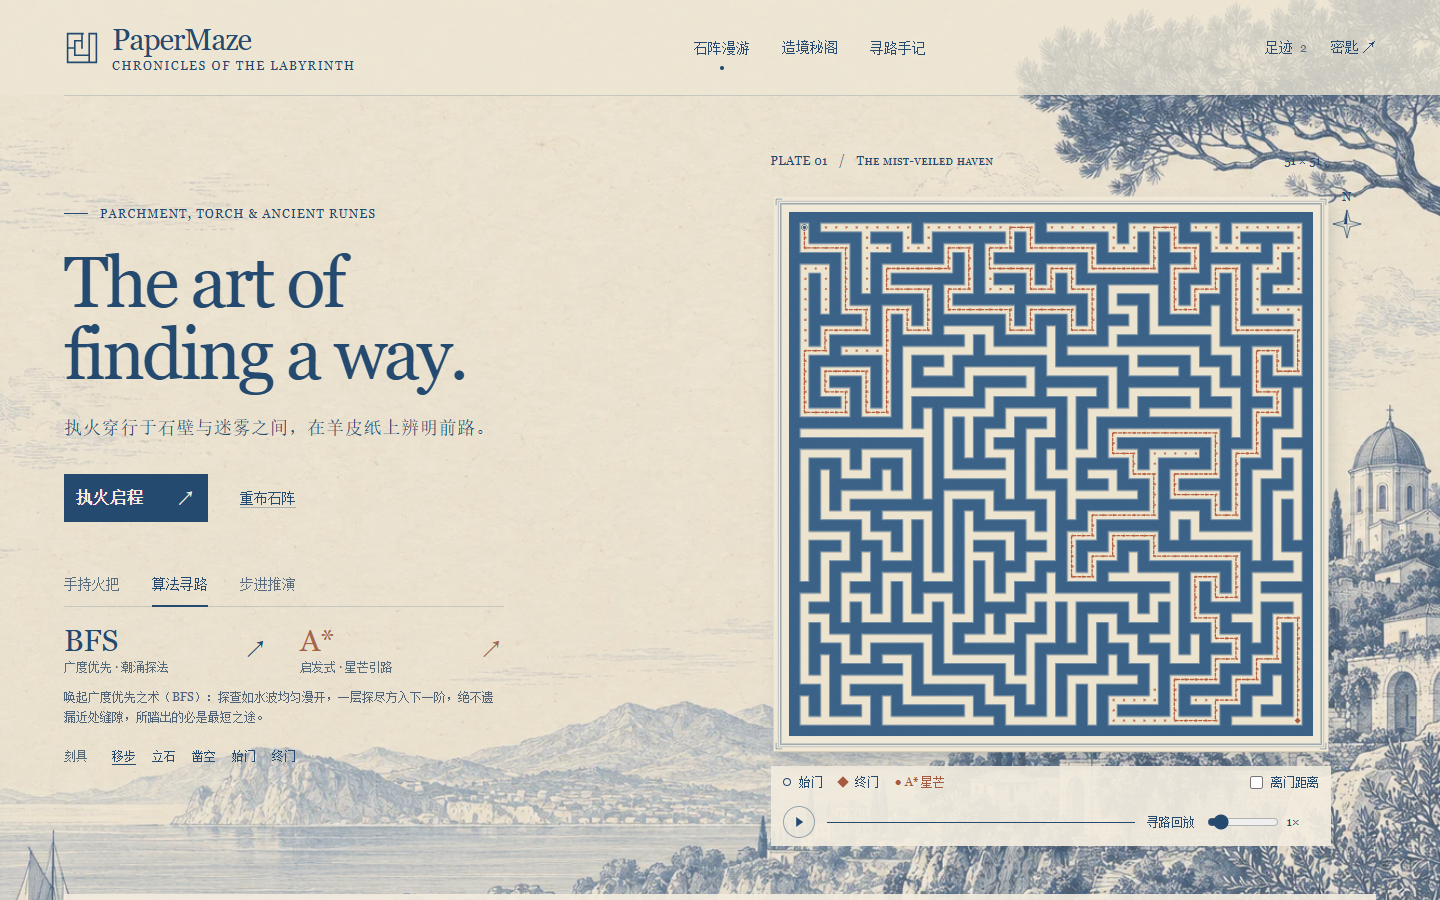
\includegraphics[width=\textwidth,height=0.46\textheight,keepaspectratio]{08-最大地图.png}
  \caption{51×51、种子12345的 A* 实际运行}
  \label{fig:largest}
\end{figure}
图\ref{fig:largest} 展示了系统在支持的最大规格（51×51，种子12345）下的单次运行表现：A* 返回372步路径，访问500个节点，页面和保存接口完成响应，未报告脚本错误。该轮还检查390px窗口无横向溢出，但没有重新执行全部历史浏览器场景。

测试期间未直接向真实外部 DeepSeek 接口发起远程网络调用，本地降级机制与网络异常模拟测试通过并不等同于完成了上游云端服务的联调整体验收。本文档引用的各项测试数据与结论均出自已有项目报告；本次文档任务的编译检查与这些历史应用验收分开说明。

\subsection{运行与复核方式}
运行环境需就绪 Windows 操作系统、Python 3.11 或更高版本、Node.js 20.19.x 或 22.12 及以上版本、pnpm 工具链，以及 Chrome 或 Edge 现代浏览器。在项目根目录下执行启动脚本（初次执行时拉取依赖需连接网络）：
\begin{lstlisting}
.\start.ps1
\end{lstlisting}
启动完成后，使用浏览器访问 \url{http://127.0.0.1:8000}，保持终端前台运行，需终止服务时按下 Ctrl+C 即可。历史数据库默认落盘在本地工程根目录下，不纳入源码版本控制。在已装配完整依赖的环境中，可执行以下命令复核自动化测试与构建：
\begin{lstlisting}
cd frontend
pnpm test
pnpm typecheck
pnpm build
cd ..
.\.venv\Scripts\python.exe -m pytest backend\tests -q
\end{lstlisting}
执行人工复核时，应至少完整演练一次“编辑迷宫—运算并保存—刷新浏览器或重启服务—恢复记录—比对矩阵数据与起终点”的持久化全流程，不能仅凭保存接口成功就认定恢复正确。

\section{AI 辅助开发说明}

\subsection{开发阶段的使用范围与责任}
在系统开发阶段，项目借助 Codex 辅助完成需求拆解、开源项目调研、技术架构选型对比、测试用例规划、基础代码初稿编写及开发文档结构梳理。在前端改版过程中，利用设计工具与动效工具辅助规划信息层级、交互状态及场景转场；海港、月桂庭院与神殿场景插画采用图像生成工具辅助构建，经转换为 WebP 格式后作为静态视觉资源引入。场景插画与叙事设计独立于核心算法逻辑，不影响寻路计算结果。

开发者负责确认需求、选择方案、理解模块输入输出和算法，并通过测试、类型检查、生产构建及浏览器验收核对生成内容。相关提示词与交互记录节选可查阅提交材料中的《AI辅助对话记录》。AI 输出不替代运行结果，也不能作为未经验证的正确性结论。

\subsection{运行时 AI 解读的边界}
运行时解读功能由后端服务端读取环境变量 \texttt{DEEPSEEK\_API\_KEY} 后，向 DeepSeek Chat Completions 接口提交校验后的寻路实验数据，密钥不发送给浏览器。默认模型为 \path{deepseek-flash}。请求采用非流式方式，禁用推理思考过程，约束最大输出长度，并设置8秒超时控制。

当环境变量未配置密钥、网络连接超时、上游接口报错或响应格式畸变时，后端自动降级并返回确定性的内置规则分析。AI 解读生成的文本不存入历史记录数据库，不影响路径生成、节点遍历计数或算法计时，亦不参与迷宫生成与求解运算。鉴于随附材料表明在测试周期内未实际调用外部真实接口，本设计仅明确接口协议与降级容灾设计，不主张已完成针对外部服务的端到端联调验收。

\section{总结}
PaperMaze 围绕迷宫生成、手动探索、BFS/A* 寻路、过程可视化与本地持久化，建立了可现场演示的完整流程。设计重点是保持地图快照不可变、隔离各次搜索状态、分离计算与播放，并以真实运行结果派生指标。

完整地图载荷解决了编辑后状态无法仅凭种子恢复的问题；前后端校验、无解处理、保存重试及 AI 降级，使辅助能力失败时不阻断主流程。带环地图的 A* 回归案例也说明，算法正确性应以固定反例和可重复测试核对，而不能只观察生成迷宫上的演示效果。

交付范围仍为本机单用户课程原型。测试结论与截图适用于材料记录的版本与场景；真实外部 AI 调用及未重跑的历史浏览器场景保留明确边界，不扩大为未验证的能力声明。

\end{document}
